\pagebreak\section{Data logger for studying charging and discharging of RC circuit}

\subsection{Experiment URL}
    Use this \href{https://www.tinkercad.com/things/awg0vQADVPP?sharecode=lBK08ktzr9HdJWinGq0Pj3PSK_MzsvQ5bzUg1wqTPac}{link} to get the \textbf{Tinkercad} simulation of this experiment.
    
\subsection{Objectives}
If a capacitor of capacitance C (in farads), initially charged to a potential $V_0$ (volts) is connected across a resistor R (in ohms), a time-dependent current will flow according to Ohm’s law. This situation is shown by the RC (resistor-capacitor) circuit below when the switch is closed.  As the current flows, the charge q is depleted, reducing the potential across the capacitor, which in turn reduces the current. This process creates an exponentially increasing voltage, modeled by
    \begin{equation}
        V_C(t)=V_0(1−e^{-\frac{t}{R.C}})
    \end{equation} 
The rate of the decrease is determined by the product RC, known as the time constant of the circuit. A large time constant means that the capacitor will discharge slowly.  The same time constant RC describes the rate of charging as well as the rate of discharging. The graph shows how the voltage across the capacitor $V_C$ and the voltage across the resistor $V_R$ vary with time when charging. The relationships are found by integrating the expression for the voltage on a capacitor. The voltage over the resistor while charging is given by:                                  
    \begin{equation}
        V_R(t)=V_0(e^{-\frac{t}{R.C}})
    \end{equation} 

We will be using a square wave voltage supply to provide the ‘switching’ between open and closed for our RC circuit. We will then examine the plots in LoggerPro of the voltages over both the capacitor and the resistor for the charging and discharging of the RC circuit. We will compare the curve fits to the theoretical predictions for the voltage and the time constant for the circuit.

The main objective of this Arduino investigation of the RC circuit is the experimental verification of the formulas for the time-varying voltage and electric current for the charging or discharging capacitor. A secondary objective is to provide an alternative to more expensive commercial laboratory materials and, at the same time, to expose the students to the underlying electronics and computer programming that would have otherwise been hidden from sight.

\subsection{Necessary Components}
We will need the following components −
\begin{itemize}
\item 1 x Arduino Uno R3
\item 1 x Breadboard
\item 1 x 100 $\mu$F capacitor
\item 1 x 10k $\Omega$ resistor
\item 1 x USB A-B cable
\item Jumper Wires
\end{itemize}

\subsection{Circuit Diagram}
            \begin{center}
            \includegraphics[width =0.85\textwidth]{images/RC_charging_discharging_circuit.png}
            \end{center}


\subsection{Arduino Code}

\begin{lstlisting}[style = Arduino]
/*DataLogger for charging and discharging of the RC Circuit */
int chargePin = 8;
int capPin = A5;

const float C = 100.0; //capacitance in uF
const float R = 10.0; //capacitance in kOhms
const float timeConstant = (R*C)/1000;

float startTimeCharge;
float startTimeDischarge;
float elapsedTimeCharge;
float elapsedTimeDischarge;
float rawInput;
float voltage;
float percentCharge;

void setup() {
  Serial.begin(9600); 
  Serial.print("The time constant of the RC circuit is: ");
  Serial.print(timeConstant);
  Serial.println("s");
  
  pinMode(chargePin, OUTPUT);
  digitalWrite(chargePin, LOW);
}

void loop() {
  rawInput = analogRead(capPin);
  voltage = (rawInput/1024.0)*5; 
  
  /////////Charging/////////////
  
  digitalWrite(chargePin, HIGH); 
  startTimeCharge = millis(); //
    
  
  while (rawInput < 1023.0) {
  rawInput = analogRead(capPin);
  voltage = (rawInput/1024.0)*5;
  float elapsedTimeCharge = (millis() - startTimeCharge) / 1000.0;  //  
  Serial.print(voltage, 3); // voltage in Volts 
  Serial.print("\t");
  Serial.print(elapsedTimeCharge, 3); //time in seconds 
  Serial.print("\n");
  delay(100);   
  }
  
 /////////Discharging/////////////
  
  digitalWrite(chargePin, LOW); 
  startTimeDischarge = millis(); //
  
  
  while (rawInput > 0.0) {   
  rawInput = analogRead(capPin);
  voltage = (rawInput/1023.0)*5;
  float elapsedTimeDischarge = (millis() - startTimeDischarge) / 1000.0;    
  Serial.print(voltage, 3); // voltage in Volts 
  Serial.print("\t");
  Serial.print(elapsedTimeDischarge, 3); //time in seconds 
  Serial.print("\n");
  delay(100);   
  }
}
\end{lstlisting}

\subsection{Charging and discharging plot}
        \begin{figure}[!ht]
            \centering
            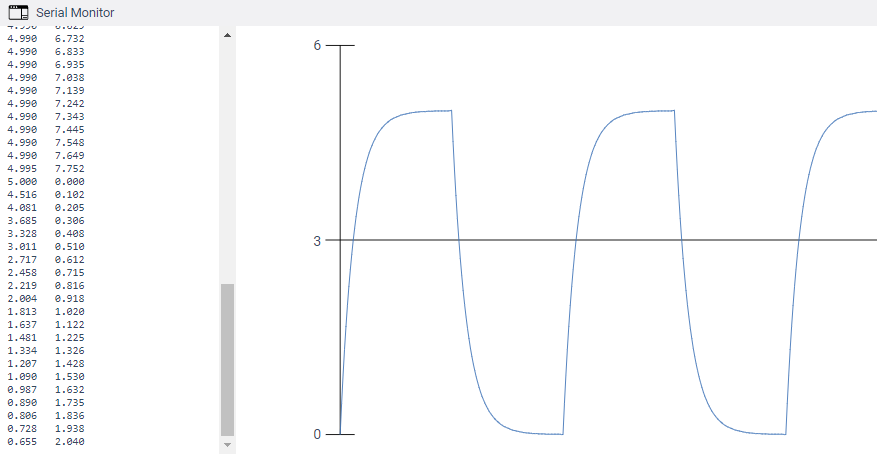
\includegraphics[width =0.85\textwidth]{images/rc_realtime_plot.png}
            \caption{Data logging real time charging and discharging}
        \end{figure}
We copied and pasted the two columns (voltage and time) of the serial monitor in a text file and plotted the data using \textbf{Python}'s plotting library \textbf{Matplotlib}.

\vspace{10pt} \begin{lstlisting}[language = Python]
import matplotlib.pyplot as plt
import numpy as np

voltage = []
time = []

#X, Y = np.loadtxt("capacitor_charging.txt", delimiter=',', unpack=True)
f = open("capacitor_discharging.txt","r")
i = []

for i in f:
    i = i.replace('\n', ' ')
    i = i.replace('\t', ' ')
    i = i.split()
    voltage.append(float(i[0]))
    time.append(float(i[1]))
print(voltage)
print(time)
plt.plot(time, voltage, "--", label = "voltage vs time")
plt.title('Capacitor Disharging')
plt.xlabel('Time (s)')
plt.ylabel('Voltage (V)')
plt.legend()
plt.show()
\end{lstlisting}

        \begin{wrapfigure}{c}{\textwidth}
            \centering
            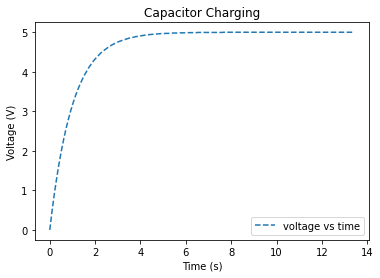
\includegraphics[scale=0.5]{images/rc_charging_plot.png}
            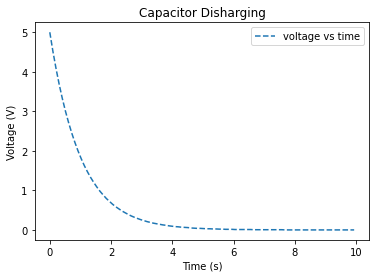
\includegraphics[scale=0.5]{images/rc_discharging_plot.png}
            \caption{RC Charging and discharging plot}
        \end{wrapfigure}

